\section{Results}

\subsection{Generic primary benchmark}
We first pool the three nonconserving circuit families across the four datasets and 20 seeds, giving 240 paired cases per method. Table~\ref{tab:generic} reports descriptive pooled means. Cross-fitted aligned AQNG has the lowest mean test loss and the highest mean test accuracy, but the margin over random-rank AQNG is small. The result therefore supports useful accessible preconditioning without supporting a universal claim that tangent alignment is always the best readout design.

\begin{table}[t]
\centering
\caption{Pooled generic primary benchmark over 240 cases. Lower test loss and higher accuracy are better.}
\label{tab:generic}
\begin{tabular}{lcc}
\toprule
Method & Test loss & Accuracy \\
\midrule
AQNG-aligned  & \textbf{0.5945} & \textbf{0.7947} \\
AQNG-random   & 0.5956 & 0.7914 \\
SGD           & 0.6084 & 0.7858 \\
Adam          & 0.6203 & 0.7731 \\
AQNG-physical & 0.6229 & 0.7878 \\
AQNG-$Z_0$    & 0.6352 & 0.7828 \\
Full-QNG      & 0.6562 & 0.7689 \\
Block-QNG     & 0.6781 & 0.7606 \\
\bottomrule
\end{tabular}
\end{table}

Cellwise outcomes remain architecture and dataset dependent, and the gap between aligned AQNG, random AQNG, SGD, and Adam is much smaller than the gap to full- and block-QNG in this common protocol. The main conclusion from the primary matrix is comparative rather than absolute: an accessible metric can preserve competitive optimization performance while exposing which measurement subspace supplies the preconditioning geometry.

\subsection{Rank baseline and qubit scaling}
The scaling experiment gives a clean geometric check of the readout-rank theory. For SU(2)--Haar circuits, the rank baseline $r/N$ decreases rapidly with $n$, while a random rank-matched readout stays near $\rho=1$. In contrast, both the physical and cross-fitted aligned readouts become increasingly super-baseline. As shown in Fig.~\ref{fig:scaling_geometry}, aligned normalized retention grows from approximately $1.62$ at $n=4$ to $30.66$ at $n=10$.

\begin{figure}[t]
\centering
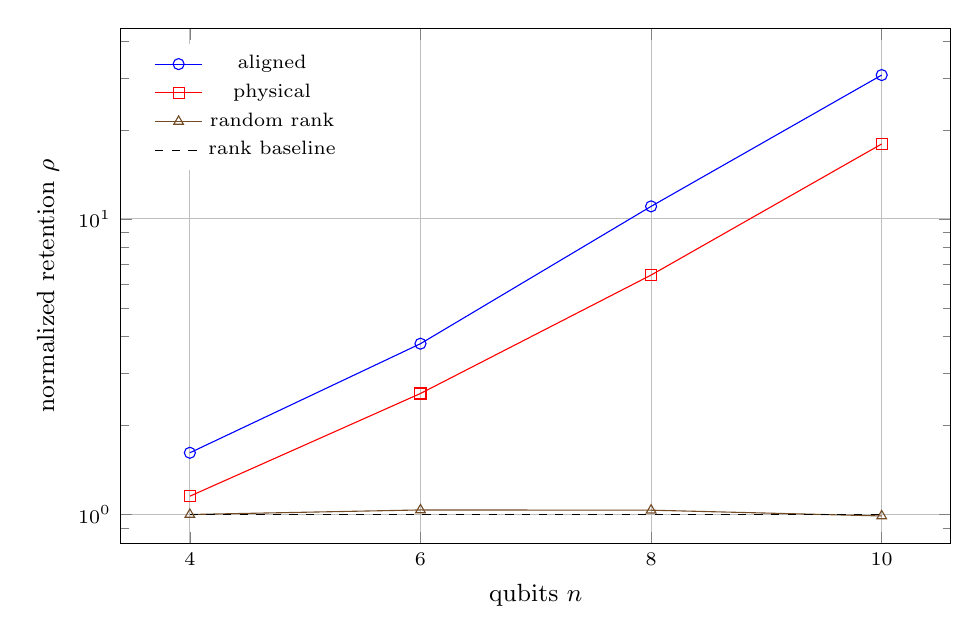
\begin{tikzpicture}
\begin{axis}[
  width=\columnwidth,
  height=0.67\columnwidth,
  ymode=log,
  xlabel={qubits $n$},
  ylabel={normalized retention $\rho$},
  xtick={4,6,8,10},
  ymin=0.8,
  legend style={draw=none, font=\scriptsize, at={(0.03,0.97)}, anchor=north west},
  tick label style={font=\scriptsize},
  label style={font=\small},
  grid=major
]
\addplot+[mark=o] coordinates {(4,1.6197) (6,3.7867) (8,11.0282) (10,30.6551)};
\addlegendentry{aligned}
\addplot+[mark=square] coordinates {(4,1.1553) (6,2.5694) (8,6.4607) (10,17.9297)};
\addlegendentry{physical}
\addplot+[mark=triangle] coordinates {(4,1.0016) (6,1.0379) (8,1.0360) (10,0.9903)};
\addlegendentry{random rank}
\addplot+[dashed, mark=none] coordinates {(4,1) (10,1)};
\addlegendentry{rank baseline}
\end{axis}
\end{tikzpicture}
\caption{SU(2)--Haar qubit scaling. The random rank-matched control remains close to $\rho=1$, whereas the structured readouts become increasingly super-baseline with system size.}
\label{fig:scaling_geometry}
\end{figure}

This strong geometric orientation does not translate into a monotonic optimization advantage. The aligned mean test losses at $n=4,6,8,10$ are $0.221$, $0.237$, $0.168$, and $0.254$, respectively. The corresponding physical-readout losses are $0.207$, $0.273$, $0.238$, and $0.241$. Thus aligned AQNG is best at $n=6$ and $n=8$, but not at $n=4$ or $n=10$. Accessibility can therefore increase relative to the null baseline while task utility remains nonmonotonic.

\subsection{Matched large/deep comparison with Adam and SGD}
The large/deep extension is a post-hoc exploratory comparison that supplies first-order baselines at $(n,L)=(8,3),(10,3),(6,5)$ for SU(2)--Haar on Iris. Table~\ref{tab:large_deep} combines the matched five-seed means. The pooled 15-case loss is $0.1867$ for aligned AQNG, compared with $0.1961$ for random AQNG, $0.2207$ for physical AQNG, $0.2268$ for Adam, $0.3998$ for SGD, and $0.4312$ for full QNG.

\begin{table}[t]
\centering
\caption{Mean test loss in the matched large/deep comparison.}
\label{tab:large_deep}
\begin{tabular}{lccc}
\toprule
Method & $n=8,L=3$ & $n=10,L=3$ & $n=6,L=5$ \\
\midrule
AQNG-aligned  & \textbf{0.168} & 0.254 & 0.139 \\
AQNG-random   & 0.210 & 0.252 & \textbf{0.127} \\
AQNG-physical & 0.238 & \textbf{0.241} & 0.183 \\
Adam          & 0.231 & 0.265 & 0.184 \\
SGD           & 0.425 & 0.407 & 0.367 \\
Full-QNG      & 0.476 & 0.430 & 0.388 \\
\bottomrule
\end{tabular}
\end{table}

In the pooled paired analysis, aligned AQNG beats SGD in 15/15 cases and full QNG in 14/15. The Holm-adjusted Wilcoxon values are $p_{\rm Holm}=1.22\times10^{-3}$ against SGD and $5.80\times10^{-3}$ against full QNG. Against Adam, aligned AQNG wins 10/15 cases with a mean loss advantage of $0.0400$, but the Holm-adjusted test is not significant. Within this exploratory extension, aligned AQNG has significantly lower paired loss than SGD and full QNG after Holm correction, while the difference from Adam is not statistically resolved.

\subsection{More retained geometry can hurt}
The readout-order ablation provides a direct counterexample to the idea that maximizing retained tangent mass is sufficient. On Iris/SU(2)--Haar, increasing the diagonal readout from weight one to weight two raises aligned retention from $0.361$ to $0.797$, yet mean test loss worsens from $0.237$ to $0.361$. On Digits/SU(2)--Haar, aligned retention rises from $0.308$ to $0.738$, while loss worsens from $0.620$ to $0.716$. Figure~\ref{fig:readout_order_tradeoff} shows the same tradeoff directly. The first-step quantity $g^{\mathsf T}d$ simultaneously drops from $7.05$ to $2.57$ on Iris and from $3.82$ to $1.71$ on Digits. Metric diagnostics show that the richer readout is substantially harder to condition. These results motivate condition-aware rather than retention-maximizing readout design.

\begin{figure}[t]
\centering
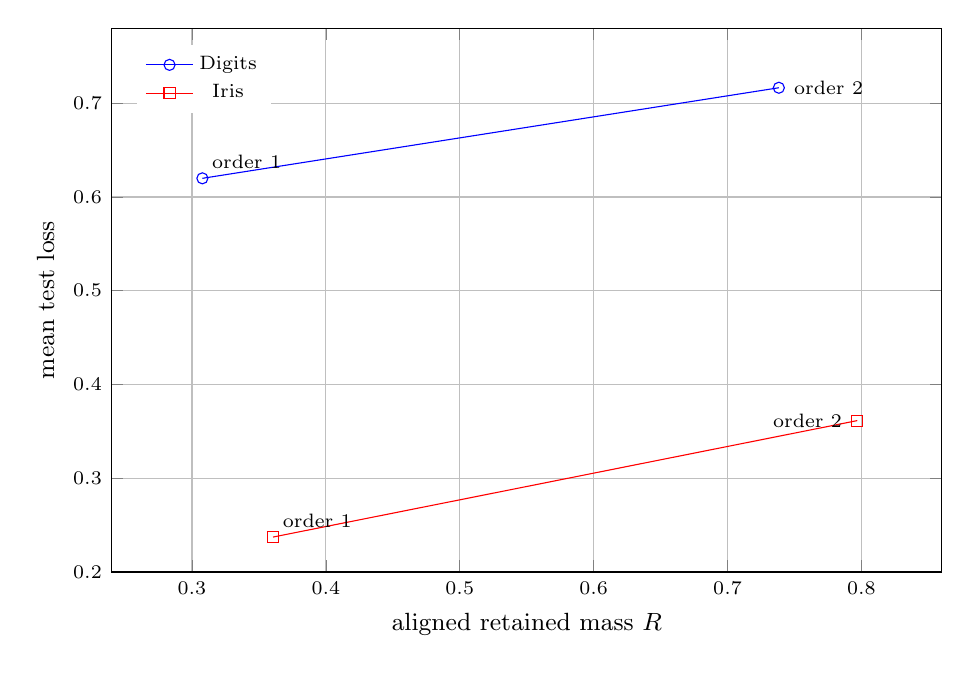
\begin{tikzpicture}
\begin{axis}[
  width=\columnwidth,
  height=0.70\columnwidth,
  xlabel={aligned retained mass $R$},
  ylabel={mean test loss},
  xmin=0.24, xmax=0.86,
  ymin=0.20, ymax=0.78,
  legend style={draw=none, font=\scriptsize, at={(0.03,0.97)}, anchor=north west},
  tick label style={font=\scriptsize},
  label style={font=\small},
  grid=major
]
\addplot+[mark=o] coordinates {(0.3078,0.6199) (0.7383,0.7165)};
\addlegendentry{Digits}
\addplot+[mark=square] coordinates {(0.3606,0.2373) (0.7969,0.3615)};
\addlegendentry{Iris}
\node[font=\scriptsize, anchor=south west] at (axis cs:0.3078,0.6199) {order 1};
\node[font=\scriptsize, anchor=west, xshift=2pt] at (axis cs:0.7383,0.7165) {order 2};
\node[font=\scriptsize, anchor=south west] at (axis cs:0.3606,0.2373) {order 1};
\node[font=\scriptsize, anchor=east, xshift=-2pt] at (axis cs:0.7969,0.3615) {order 2};
\end{axis}
\end{tikzpicture}
\caption{Readout-order tradeoff for aligned AQNG on SU(2)--Haar. Moving from weight-one to weight-two diagonal readouts increases retained tangent mass but also increases mean test loss on both datasets.}
\label{fig:readout_order_tradeoff}
\end{figure}

\subsection{Accessibility does not imply trainability}
The number-conserving $U(1)$ family is the strongest negative control. Its physical and aligned readouts remain nearly maximally accessible as system size grows: at $n=8$, aligned retention is $0.99993$, and at $n=10$ it is $0.99987$. Nevertheless, all tested optimizers approach the same chance-like accuracy of $0.4667$ at $n=8$ and $n=10$, with terminal loss near $2.1333$. At the same time, the recorded first-step descent signal collapses by many orders of magnitude. Figure~\ref{fig:u1_signal} contrasts the small accessibility deficit $1-R_{\rm aligned}$ with the rapidly vanishing first-step $g^{\mathsf T}d$. The failure is therefore not measurement blindness; the supervised optimization signal itself becomes too weak to exploit.

\begin{figure}[t]
\centering
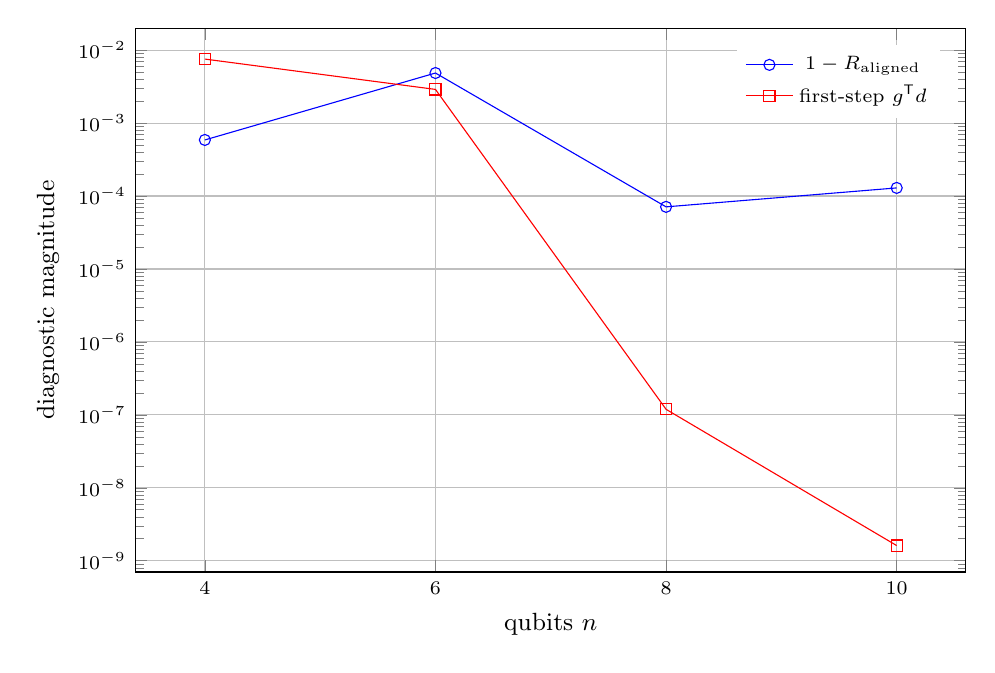
\begin{tikzpicture}
\begin{axis}[
  width=\columnwidth,
  height=0.70\columnwidth,
  ymode=log,
  xlabel={qubits $n$},
  ylabel={diagnostic magnitude},
  xtick={4,6,8,10},
  ymin=7e-10, ymax=2e-2,
  legend style={draw=none, font=\scriptsize, at={(0.97,0.97)}, anchor=north east},
  tick label style={font=\scriptsize},
  label style={font=\small},
  grid=major
]
\addplot+[mark=o] coordinates {(4,5.878e-4) (6,4.863e-3) (8,7.109e-5) (10,1.293e-4)};
\addlegendentry{$1-R_{\rm aligned}$}
\addplot+[mark=square] coordinates {(4,7.554e-3) (6,2.898e-3) (8,1.191e-7) (10,1.614e-9)};
\addlegendentry{first-step $g^{\mathsf T}d$}
\end{axis}
\end{tikzpicture}
\caption{Diagnostic separation in the number-conserving $U(1)$ scaling control. The aligned readout remains nearly complete, while the first-step descent signal collapses by several orders of magnitude.}
\label{fig:u1_signal}
\end{figure}

This regime is consistent with the gradient-concentration phenomenology associated with barren plateaus~\cite{McClean2018}, but we do not claim a formal barren-plateau scaling theorem: the scaling study uses five seeds and was not designed to estimate an exponential gradient-variance law over a large initialization ensemble. The directly observed conclusion is narrower: near-complete measurement accessibility does not rescue a vanishing task-signal regime.

\subsection{Finite-shot robustness}
At 1000 and 10000 shots, AQNG remains operational across the tested Iris and Digits SU(2)--Haar cells. For example, on Digits the aligned losses are $0.661$ and $0.624$ at 1000 and 10000 shots, respectively, compared with $0.829$ and $0.790$ for the full-QNG control. On Iris, random-rank AQNG is the best of the tested AQNG variants at both shot counts. The ordering is therefore not monotonic in shot count or readout orientation. Because the finite-shot full-QNG implementation uses an analytic metric oracle, these numbers are optimization references rather than a resource-fair hardware comparison.
